\chapter{Compilation depuis la source} 
\minitoc
\label{ssse:compilation-source}

\clearpage


\section{Introduction}
Comme nous l'avons évoqué, notre système sera construit entièrement à partir des sources, afin de garantir une indépendance totale vis‑à‑vis des distributions grand public. Nous devons donc étudier les mécanismes et les problématiques liés à la compilation.


\section{Qu’est‑ce qu’un paquet ?}
\label{sssec:definition-paquet}

Un \emph{paquet} est un ensemble de fichiers (bibliothèques, scripts, documentation) fournissant une fonctionnalité précise dans le système : ce paquet peut être un compilateur (\texttt{gcc}), un utilitaire de liens (\texttt{binutils}), un outil de recherche de fichiers (\texttt{findutils}), un utilitaire de base (\texttt{coreutils}), un backend de compilation (\texttt{LLVM}), etc.

Généralement, ce paquet est compressé sous un format tar.gz ,tar.xz,tar.bz2 ou zip, que l’on peut obtenir depuis le site officiel ou en clonant le dépôt GitLab/GitHub.\\
Il contient le code source  et \textbf{un système de build} décrivant comment compiler le paquet.\\ Parfois, il inclut aussi les sources de tiers nécessaires à la construction : par exemple, si le programme final executable est lié dynamiquement à \texttt{libc}, l’auteur du paquet peut inclure une version locale de \texttt{glibc}  dans ses sources.\\
\bigbreak
\textbf{Question :} Les execuatble  sont-ils liés dynamiquement ? 

Cette question est cruciale dans un système Linux et nous amène naturellement à distinguer les bibliothèques statiques et les bibliothèques partagées.

\begin{figure}[H]
  \centering
  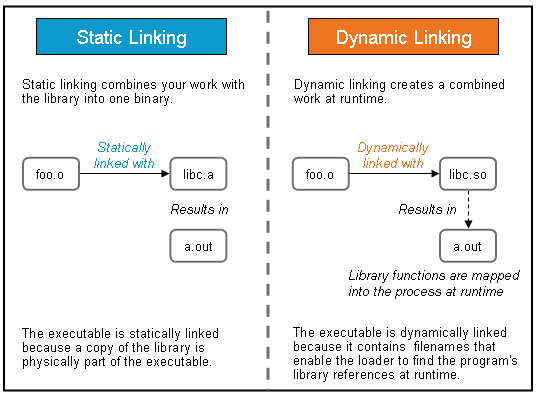
\includegraphics[width=1\textwidth]{images_pfe/sharedlibraryvsstatic.png}
  \caption{Bibliothèque statique vs partagée}
  \label{fig:staticsharedl}
\end{figure}

\paragraph{Bibliothèques statiques vs partagées}
\begin{enumerate}
  \item \textbf{Bibliothèques statiques} :  
    Les bibliothèques statiques sont des archives de routines (\texttt{libfoo.a}) dont les routines nécessaires sont extraites et \textbf{liées directement} dans l’exécutable.  
  \item \textbf{Bibliothèques partagées (dynamiques)} :  
    Les bibliothèques partagées (\texttt{libfoo.so}) sont chargées une seule fois en mémoire virtuelle, puis \textbf{partagées} par tous les programmes qui les utilisent. Elles sont plus économes en espace.\\
\end{enumerate}





\textbf{Exemple d'un exécutable lié statiquement : Hello World en FASM (Flat Assembleur)}

\begin{figure}[H]
  \centering
  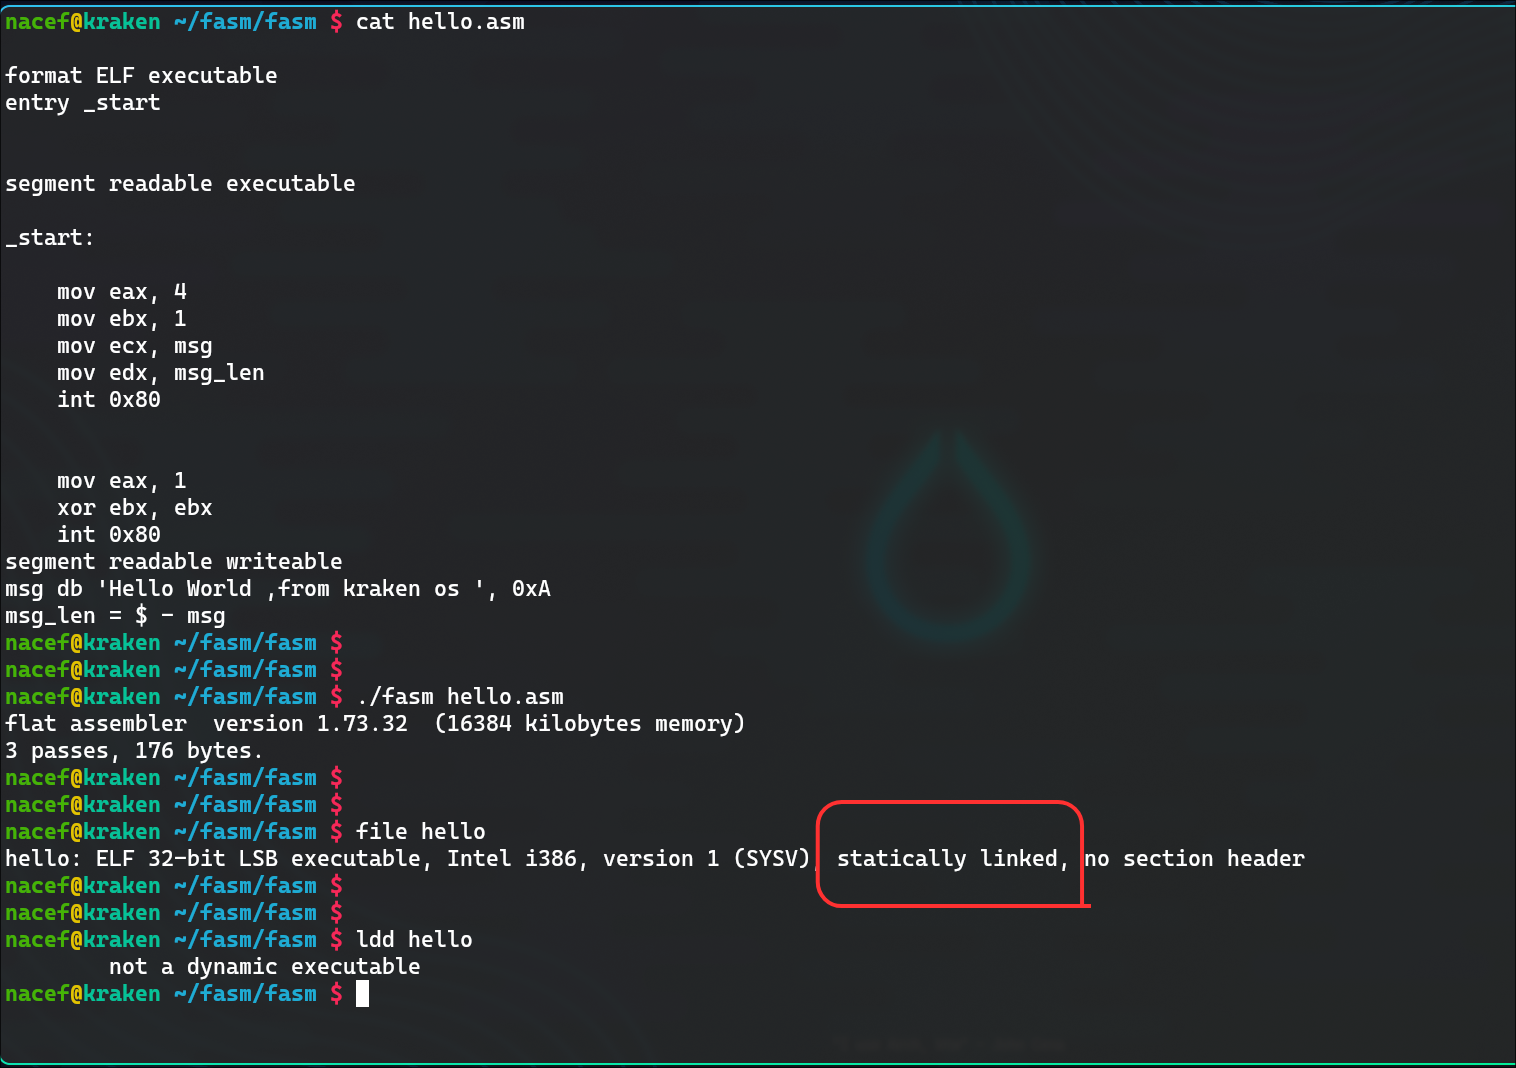
\includegraphics[width=1\textwidth]{images_pfe/staiclulinkedoff.png}
  \caption{Exécutable lié statiquement }
  \label{fig:staticsharedl}
\end{figure}
\clearpage

\textbf{Exemple d'un exécutable lié dynamiquement : Hello World en C }
\begin{figure}[H]
  \centering
  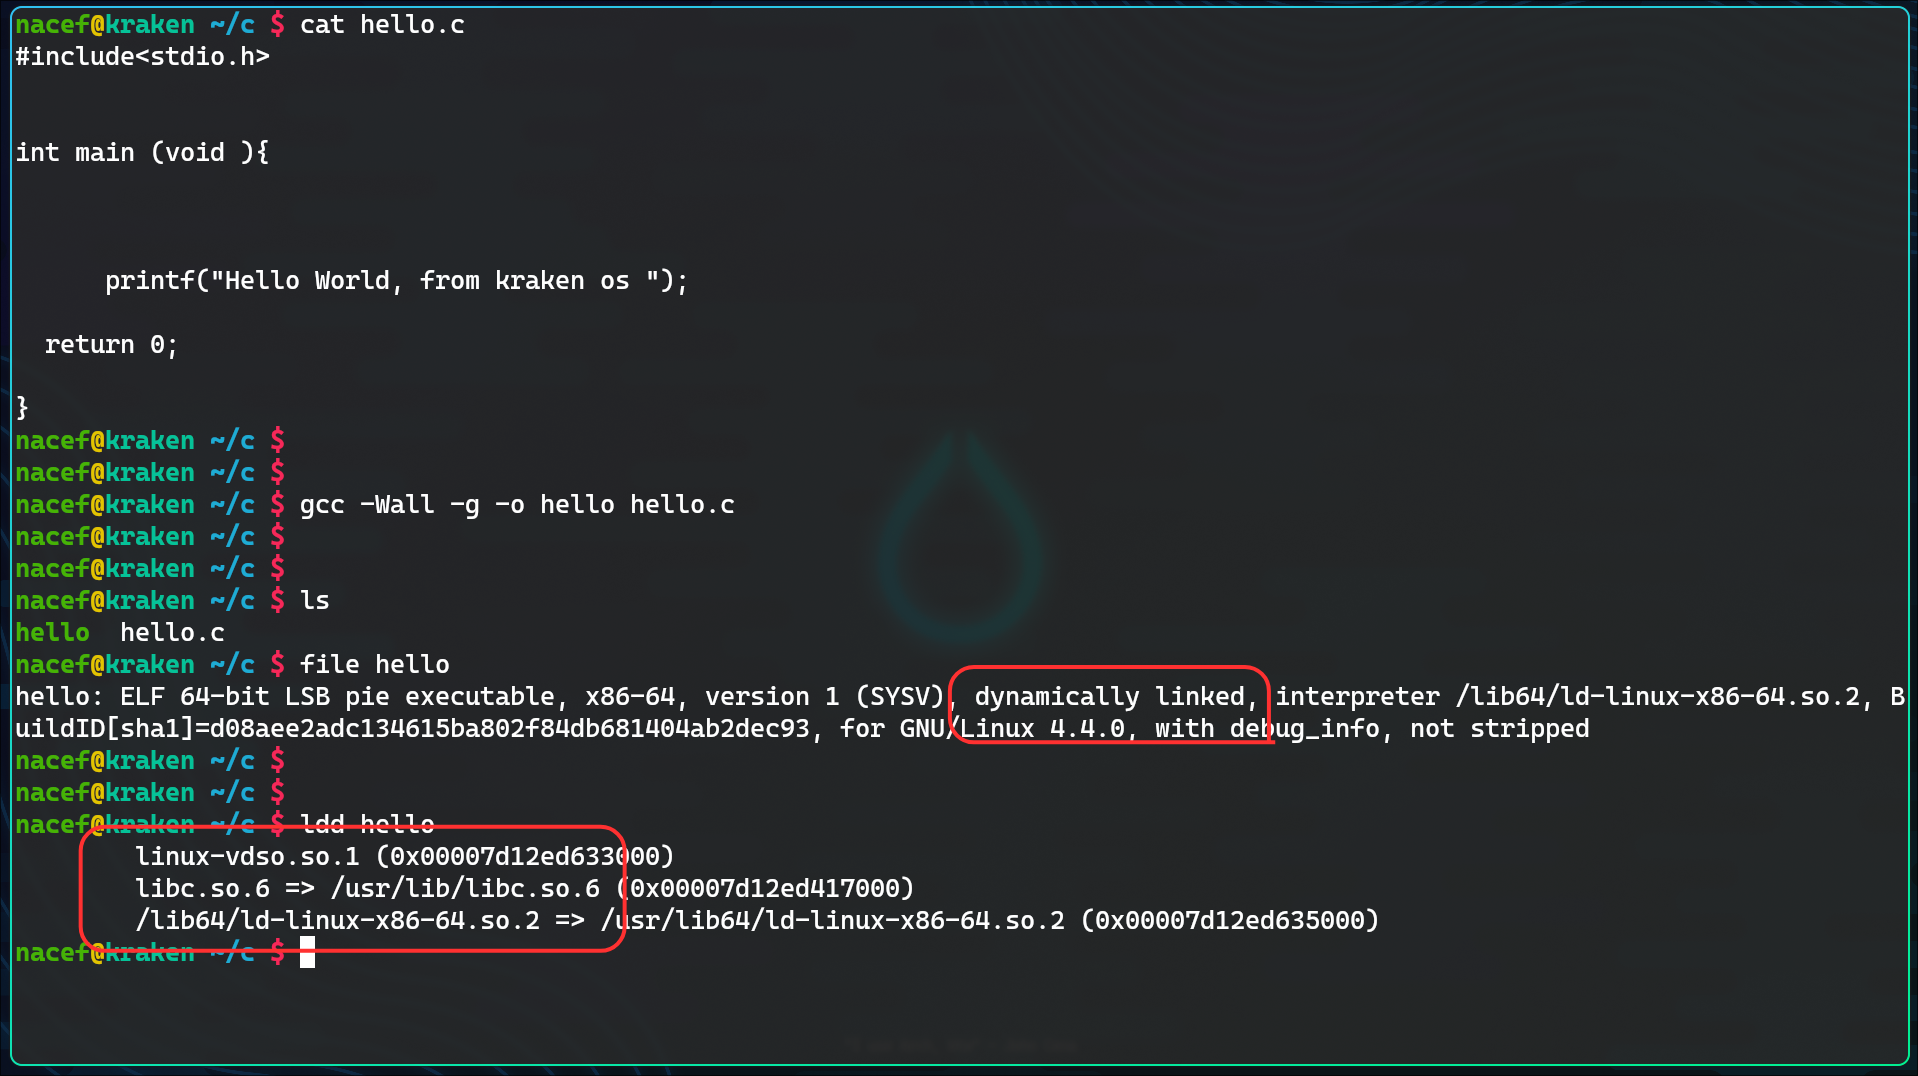
\includegraphics[width=1\textwidth]{images_pfe/dynamiclinkedoff.png}
  \caption{Exécutable lié dynamiquement }
  \label{fig:staticsharedl}
\end{figure}





\paragraph{Remarque}  
En général, les mainteneurs développent ces paquets pour une distribution spécifique (Arch, Debian, etc.). Pour les adapter à  notre distribution, il est parfois nécessaire d’appliquer des patches ou de modifier les chemins dans le code source, car l’emplacement des bibliothèques peut varier d’une distribution à l’autre.  \\
Par exemple, si un paquet s’attend à trouver la bibliothèque \texttt{libX} dans \texttt{/lib} mais que nous l’installons dans \texttt{/usr/lib}, il faudra créer un lien symbolique ou ajuster le chemin de recherche durant le build.  Ce problème est appelé \textbf{erreurs de liaison} (Link Errors)






\section{Qu’est‑ce que la compilation à partir des sources ?}
\label{subsec:compilation-sources}


Un système d’exploitation open‑source est le fruit de l’intelligence collective ; chaque ligne de code est accessible et modifiable. L’installation à partir des sources requiert donc de parcourir les sources de chaque paquet et de les compiler soi‑même pour générer les exécutables, la documentation, les bibliothèques, etc.

Généralement, cette étape de compilation s’effectue en utilisant le \textbf{système de build} propre à chaque paquet.

\subsection{Qu’est‑ce qu’un système de build ?}
\label{sssec:definition-buildsystem}

Un \emph{système de build} est l’outil ou l’ensemble d’outils orchestrant la configuration, la compilation, le lien et l’installation des sources. Parmi les plus courants :

\begin{table}[H]
    \centering
    \begin{tabular}{|c|c|p{8cm}|}
        \hline
        \textbf{Logo} & \textbf{Outil} & \textbf{Fonction principale} \\
        \hline
        
\includegraphics[width=0.8cm]{images_pfe/make.png} & Make & Le plus ancien et basique, utilise des Makefiles. \\
        \hline
        
\includegraphics[width=0.8cm]{images_pfe/GNU-Autoconf-768x288.jpg} & Autotools & Traditionnel pour projets open source, gère la compilation croisée. \\
        \hline
        
\includegraphics[width=0.8cm]{images_pfe/zig.png} & Zig & Outil intégré à Zig (compilation C/C++ possible). \\
        \hline
        
\includegraphics[width=0.8cm]{images_pfe/meson_logo.png} & Meson & Alternative moderne et rapide à CMake/Autotools. \\
        \hline
        
\includegraphics[width=0.8cm]{images_pfe/ninja.jpeg} & Ninja & Outil bas niveau, très rapide, utilisé comme backend pour CMake/Meson. \\
        \hline
    \end{tabular}
    \caption{Principaux systèmes de build}
    \label{tab:build_tools_logos}
\end{table}


%------------------------------------------------
\subsection{Étapes générales de compilation}
\label{sssec:etapes-compilation}

Lors de la construction du système, nous compilons des dizaines de bibliothèques, paquets, etc. Il est donc nécessaire de comprendre comment fonctionne le processus de compilation :

\begin{enumerate}
  \item \textbf{Collecte d’informations}  
    Lire la documentation officielle (wiki, dépôt GitHub/GitLab) pour connaître les dépendances et les options de compilation.\\
    

  \item \textbf{Récupération du code source}  
    Télécharger l’archive (\texttt{.tar.gz}, \texttt{.zip}) à l’aide d’outils tels que \texttt{wget}, \texttt{curl}, ou cloner depuis le dépôt GitLab/GitHub officiel.  
   
    Vérifier ensuite l’intégrité de l’archive (car le téléchargement peut être interrompu ou corrompu),\\ 
     puis l’extraire  et contrôler son contenu (généralement les fichiers du système de build \textcolor{blue}{\ref{fig:makefileexemple}}  ).\\

 \item \textbf{Configuration}  
    À cette étape, le système de build vérifie la présence des bibliothèques, paquets et outils requis, puis active les options souhaitées.  \\

    \textbf{Remarque :} les options de configuration sont très délicates et importantes, car chaque paquet dépend des autres. Il convient donc de se poser deux questions après la configuration de chaque paquet :
    \begin{enumerate}[label=\arabic*)]
      \item Quelle est la configuration nécessaire pour assurer le bon fonctionnement de ce paquet ?
      \item Quelles options doivent être activées maintenant pour que les futurs paquets, qui dépendent de celui-ci, puissent utiliser correctement ses fonctionnalités ?
    \end{enumerate}


    \medskip
    \noindent\textbf{Exemple pratique :} \\ 
    LLVM est un compilateur backend qui gère l’IR (Intermediate Representation). Pour le compiler, il faut construire Clang  (runtime LLVM) d abord  \textbf{avec le support de}  \texttt{compiler-rt} :

    \begin{verbatim}
cmake \
  -DLLVM_ENABLE_PROJECTS="clang;compiler-rt"
    \end{verbatim}
   %Pour plus de détails sur les configurations avec des exemples , voir la section~\hyperref[sec:config-packages]{\textcolor{blue}{\ref*{sec:config-packages}}} de l'annexe.
    
  \item \textbf{Compilation}  
    Après configuration, nous lancer la construction des binaires via le
système de build 

  \item \textbf{Tests (facultatif):}  
     Generalement,après compilation nous tester le paquet, surtout s’il est critique
   
  
\item \textbf{Installation:}  
   installer les fichiers dans l’arborescence cible 

  \item \textbf{Post-configuration (documentation):}  
    Après installation, vous pouvez ajouter des étapes d'installation de documentation ou de génération de fichiers de configuration. 

  \item \textbf{Nettoyage et désinstallation:}  
    Supprimer les fichiers temporaires et le répertoire de
build, tout en conservant l’archive source pour d’éventuelles recompilations.
\end{enumerate}
\clearpage






\textbf{Exemple de fichier Makefile utilisé par le système de build \texttt{make}}\\
Nous présentons ici un Makefile minimal pour le package \texttt{construire\_graphe}, un outil simple écrit en C permettant de générer et visualiser des graphes. Chaque section du Makefile correspond à une étape du processus de compilation standard.

\begin{itemize}
  \item \textbf{Fonctionnalités clés} :
  \begin{itemize}
    \item Construction de graphes via un algorithme implémenté en C
    \item Affichage clair des résultats dans le terminal
    \item Système d’aide intégré pour guider l’utilisateur
  \end{itemize}

  \item \textbf{Composants principaux} :
  \begin{itemize}
    \item \texttt{construire\_graphe} : exécutable principal
    \item \texttt{graph.h/graph.c} : bibliothèque de manipulation de graphes
    \item \texttt{helpmenu.sh} : script d’aide interactif
  \end{itemize}
\end{itemize}

\begin{figure}[H]
  \centering
  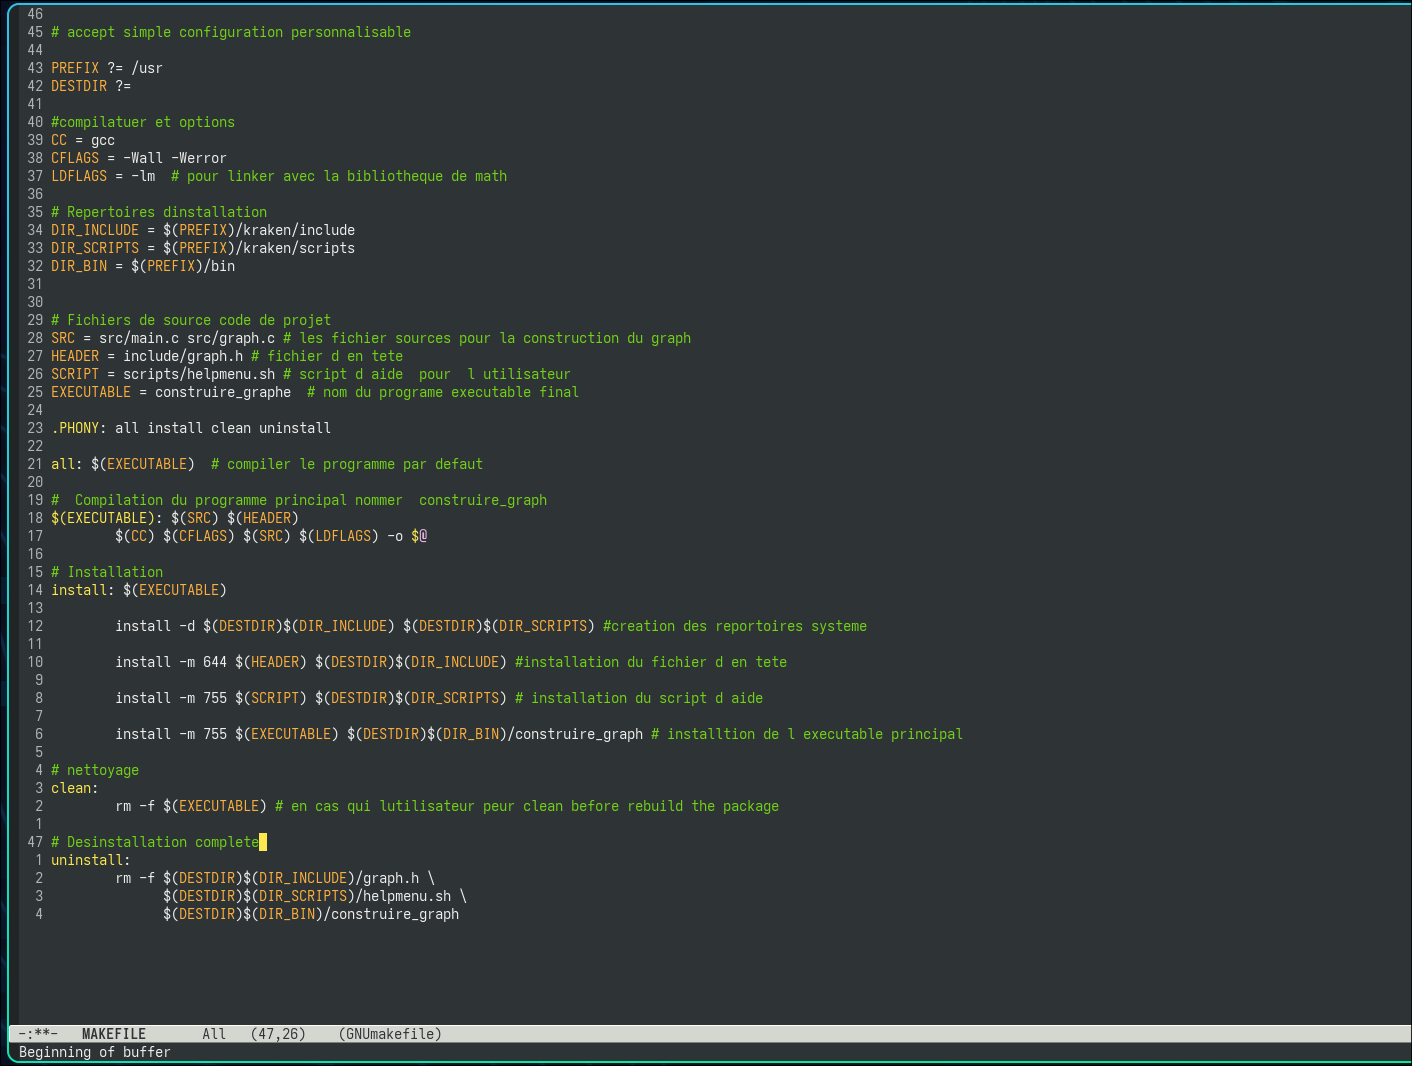
\includegraphics[width=\textwidth]{images_pfe/makefileexemple.png}
  \caption{Exemple de fichier Makefile}
  \label{fig:makefileexemple}
\end{figure}
\clearpage
Le processus de compilation avec \texttt{make} peut être résumé en six étapes clés, illustrées par notre Makefile :

\begin{enumerate}
  \item \textbf{Récupérer le code source de l’outil\\}  
    Par exemple :\\
    \begin{verbatim}
wget https://www.exemple_domain.tn/graph/releases/graph-1.0.1.tar.xz
    \end{verbatim}

  \item \textbf{Extraire l’archive}  
    \begin{verbatim}
tar -xvf graph-1.0.1.tar.xz
    \end{verbatim}

    Exemple de structure du projet :
    \begin{figure}[H]
      \centering
      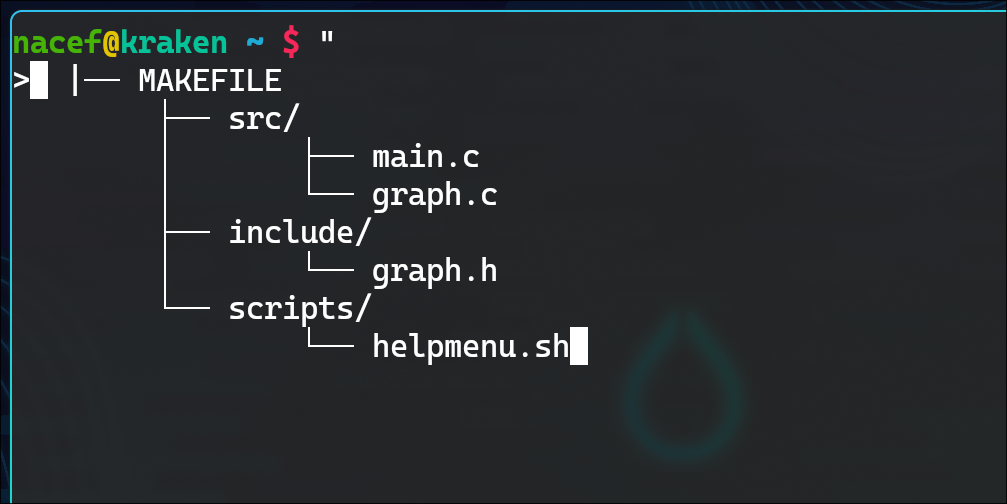
\includegraphics[width=0.7\textwidth]{images_pfe/construire_graph_structure.png}
      \caption{Structure du projet \texttt{construire\_graphe}}
      \label{fig:construire_graph}
    \end{figure}

  \item \textbf{Compilation}  
    \begin{verbatim}
make --DESTDIR=/opt
    \end{verbatim}
    Lorsque vous exécutez \texttt{make}, l’outil cherche la première cible (ici \texttt{all}), constate que \texttt{construire\_graphe} est nécessaire, puis exécute la règle correspondante :  
    \begin{verbatim}
gcc -Wall -Werror src/main.c src/graph.c -lm -o construire_graphe
    \end{verbatim}

  \item \textbf{Installation}  
    \begin{verbatim}
make DESTDIR=/opt install    
    \end{verbatim}
    Cette cible crée d’abord les répertoires d’installation :\\
    \begin{verbatim}
install -d /opt/kraken/include /opt/kraken/scripts

    \end{verbatim}
Puis copie les fichiers avec les permissions adéquates :\\

  \begin{verbatim}

install -m 644 graph.h          /opt/kraken/include
install -m 755 helpmenu.sh      /opt/kraken/scripts
install -m 755 construire_graphe /opt/bin
    \end{verbatim}

  \item \textbf{Nettoyage}  
    \begin{verbatim}
make clean
    \end{verbatim}
    Avec la règle dans le Makefile :
    \begin{verbatim}

clean:
    rm -f construire_graphe
    \end{verbatim}
    Cette cible supprime l’exécutable compilé.

  \item \textbf{Désinstallation}  
    \begin{verbatim}
make uninstall
    \end{verbatim}
    Avec la règle dans le Makefile :
    \begin{verbatim}

uninstall:
    rm -f /opt/kraken/include/graph.h \\
          /opt/kraken/scripts/helpmenu.sh \\
          /opt/bin/construire_graphe
    \end{verbatim}
    Cette cible retire les fichiers installés.
\end{enumerate}

  





   
\textcolor{blue}{Pour plus d’informations sur la compilation des paquets depuis les sources, consultez} \cite{tutoriel_unix}

\section{Qu’est‑ce que le \emph{bootstrap} ?}
\label{subsec:bootstrap}
\begin{figure}[H]
  \centering
  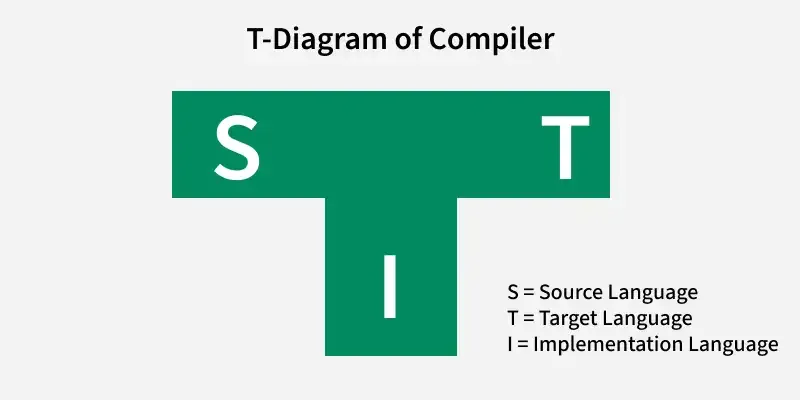
\includegraphics[width=0.85\textwidth]{images_pfe/bootstrap.png}
  \caption{Schéma de l’amorçage d’un compilateur}
  \label{fig:bootstrap}
\end{figure}

Lors de la compilation de paquets à partir des sources, nous rencontrons souvent des problèmes liés à l’amorçage (\emph{bootstrap}).  \\
Le \emph{bootstrap}  permet de compiler un composant dont le compilateur est écrit dans le même langage — et donc non disponible a priori sur la machine de construction. 

\bigskip
\noindent
\textbf{Problème}  
Supposons que l’on veuille construire le langage \texttt{Go}, dont le compilateur  est écrit en la langage  \texttt{Go} lui‑même. Comment produire un exécutable quand aucun compilateur \texttt{Go} n’est encore installé ?

\medskip
\noindent
\textbf{Solution}  
On utilise un \emph{bootstrap} : un binaire pré‑compilé ou un compilateur antérieur sert à générer la première version du compilateur \texttt{Go}. Ce compilateur issu du bootstrap est ensuite utilisé pour compiler la version finale.  \\
Vous pouvez simplement comprendre ce concept comme « compiler un compilateur à l’aide d’un compilateur préexistant pour générer le compilateur définitif ! »\\



Cette méthode générale s’applique à tout langage ou outil dont le compilateur est en auto‑hospitage (\emph{self‑hosting}).( Exemple :langage go,  langage rust , language java ...) \\
\textcolor{blue}{Pour plus d’informations sur auto-hospitage, consultez \cite{bootstrap}}
%-------------------compiler ------------------
\section{Compilateur croisé}
\label{subsec:cross-compiler}

La compilation croisée est utilisée pour construire un compilateur et sa chaîne d’outils pour une machine différente de celle servant à la compilation. \\ 
Simplement pour générer des exécutables qui fonctionneront sur une machine différente de la machine hôte .\\ 
Par exemple, on peut utiliser un cross-compiler installé sur une architecture x86\_64 pour produire des exécutables destinés à l’architecture ARM .

\begin{figure}[!htbp]
  \centering
  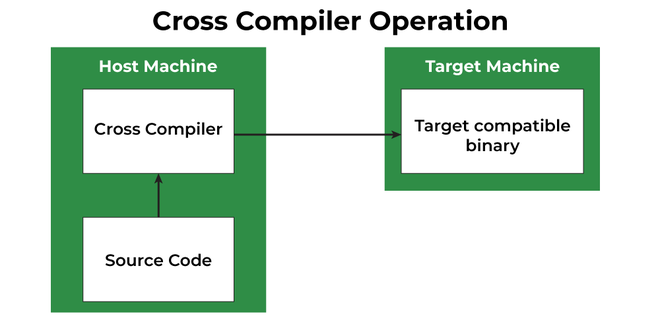
\includegraphics[width=0.85\textwidth]{images_pfe/crosscompiler.png}
  \caption{Compilateur croisé}
  \label{fig:crosscompiler}
\end{figure}

%\subsubsection{Notions clés}
%\begin{itemize}
  %\item \textbf{Build} : machine utilisée pour la compilation.
 % \item \textbf{Host} : machine sur laquelle les programmes compilés seront exécutés.
 % \item \textbf{Target} : architecture cible pour laquelle le code est généré.
%\end{itemize}


%\subsection{Exemple pratique : Canadian Cross}
%La méthode dite « Canadian Cross » se déroule en quatre étapes successives, impliquant trois machines distinctes.

%Nous disposons d'un compilateur natif sur une machine lente (machine A), appelé \texttt{ccA}. Nous disposons également d'une machine rapide (machine B) \textbf{sans compilateur}, et nous souhaitons produire du code pour une troisième machine lente (machine C).\\
%Nous allons construire un compilateur pour la machine C en quatre étapes :

%\begin{table}[!htbp]
 % \centering
 % \caption{Processus de compilation « Canadian Cross »}
 % \label{tab:canadian-cross}
 % \begin{tabular}{|l|l|l|l|p{6cm}|}
 %   \hline
 %   \textbf{Étape} & \textbf{Build}    & \textbf{Host}    & \textbf{Target}  & \textbf{Action}                                      \\
 %   \hline
 %   1              & A          & A                & B                & Compilation de \texttt{cc1}  avec \texttt{ccA} sur A    \\
 %   \hline
    %2              & A                 & B                & C                & Compilation %de \texttt{cc2} à l’aide de \texttt{cc1} sur A                \\
    %\hline
    %3              & B            & C                & C                & Compilation de \texttt{ccC} (natif) avec \texttt{cc2} sur B                \\
   % \hline
   % 4              & C                 & C                & C                & Rebuild et test de \texttt{ccC} avec lui‑même sur C                      \\
   % \hline
  %\end{tabular}
%\end{table}

%Dans cet exemple :
%\begin{itemize}
%  \item \textbf{cc1}, \textbf{cc2} : compilateurs croisés, générant du code pour une autre %architecture.
%  \item \textbf{ccA}, \textbf{ccC} : compilateurs natifs, générant du code pour leur %machine hôte.
%\end{itemize}

%\bigskip
%\noindent
\textbf{Remarque :} dans le cas de \textsc{notre distribution}, la machine hôte  et la machine cible(kraken os) sont identiques (même architecture x86-64).\\
\textbf{Pourquoi utiliser alors un compilateur croisé ?}\\
Tout simplement pour \textbf{l’isolation  :}  car  tout ce qui est compilé en croisé ne peut pas dépendre de l’environnement hôte.\\
En effet, si nous compilons nos paquets système à l’aide du compilateur du système hôte, les outils et les exécutables sont liés dynamiquement à des bibliothèques présentes sur l’hôte,Donc Les outils générés resteront dépendants de cet environnement. Ainsi, lorsque nous effectuons un chroot ou que nous démarrons notre système, tous ces exécutables produits ne fonctionneront pas

\medskip
\noindent
\textbf{Solution :}  
Nous mettrons en œuvre un « faux » cross‑compiler. Cette approche sera détaillée dans le  Section~\textcolor{blue}{\ref{subsec:build-cross}}.\\

\textcolor{blue}{Pour plus d’informations sur le compilateur croisé, consultez \cite{lfs_book} des pages 39 à 43.}  
\section{Conclusion }

Compiler un logiciel à partir des sources reste une tâche exigeante, souvent perçue comme laborieuse en raison de son \textbf{coût temporel} et de sa \textbf{complexité technique} . La configuration des paquets, les dépendances imbriquées et la compilation de projets massifs (GCC, Qt6, KDE, LLVM, Mesa, ou le noyau Linux) peuvent monopoliser des heures de calcul, même sur des machines puissantes dotées de 8 cœurs CPU.

C’est précisément pour simplifier cette démarche que les grandes distributions Linux ont développé des gestionnaires de paquets ,  mais au fait, \textbf{qu’est-ce qu’un gestionnaire de paquets ? Comment fonctionne-t-il ? }\\

C’est ce que nous découvrirons dans le prochain chapitre !